\chapter{Methodology}
	In order to find solutions for equation \ref{eq:problem}, a series of steps and decisions must
	be made. Such decisions include the modeling of the hyperparameter space and its sampling, the
	choice of the numerical optimization method, and the definition of the target function to
	optimize, among others.

	The general strategy followed here is summarized in figure \ref{fig:generalapproach}:

	\begin{figure}[here]
		\begin{center}
			%
\includegraphics{lorem}
			\missingfigure[figwidth=12cm]{Insert overall scheme here}
		\end{center}
		\caption[General methodology diagram]{Interaction between different components of the
		implemented hyperparameter optimization and model selection approach.}
		\label{fig:generalapproach}
	\end{figure}


\section{Data preprocessing}
	The training step for any SML algorithm performs analysis on a set of example instances of the
	form $(\feature, \class)$ to detect patterns or rules that enable it to predict the class of
	unseen instances. This necessarily implies that a good prediction would strongly depend on the
	numerical values in the feature vector $\feature$ and their relation with their class $\class$.

	In most real-world applications, the raw data obtained from experiments is not immediately suitable for
	training SML algorithms. Data with high dimensionality (many features) usually requires heavier computation to
	process, and the large number of dimensions can make a very informative signal (i.e., a
	dimension or group of dimensions that correlate well with the labeling) difficult to detect among
	all the rest of non-informative dimensions. Non-homogeneous scaling of the features may cause
	for certain algorithms to erroneously assume some features more relevant than others. Some
	features may only significantly contribute to a good signal for discrimination when combined
	with others.

	To address this problem, many \emph{feature selection} and \emph{dimensionality reduction}
	techniques \todo{Name feature selection techniques? (None has been included so far.)} exist\ldots


\section{Hyperparameter space modeling}
	\label{sec:hyperparam_dist}
	Most SML algorithms ship with default hyperparameter values that control different aspects of their
	internal behavior, which can be further adjusted to fit specific needs. For example, algorithms
	that make use of the distance between examples in feature space might accept a distance metric
	to be specified, or algorithms that internally create trees might allow the user to specify a
	branching factor (maximum number of branches per node), and so on.  The choice of hyperparameter
	values can heavily impact the predictive power of a SML algorithm.

	Different aspects of the hyperparameter modeling must be taken into account. Individual
	hyperparameters can be either nominal or ordinal, ordinal hyperparameters can be discrete or
	continuous, or can be valid only within a specific range. Furthermore, some hyperparameters are
	only used in combination with specific values of others and thus exhibit conditional
	dependencies.

	\subsection{Hyperparameter distributions}
	\label{ssec:hyperparam_dist}
	Since one of the main objectives of this work is to learn the behavior of SML algorithms under
	different settings, a systematic way of getting candidate configurations for performance
	evaluation is required. In order to achieve this, each hyperparameter is regarded as a random
	variable and a distribution for its specific type is assigned to it.

	A prior one-dimensional distribution is used to sample values for each hyperparameter
	independently. Section \ref{ssec:hyp_hierarchy} describes in detail how dependencies between
	hyperparameters are handled. The general approach is to create separate distributions for
	hyperparameters that depend on other categorical hyperparameters, according to the particular
	values that the category might take.

	The choice of the prior depends on the nature of each hyperparameter and the knowledge of the
	range and expected values that the hyperparameter might take. The implemented types of prior
	distributions are:
	\begin{itemize}
		\item {\bf Categorical} distributions assigned to hyperparameters that can take nominal values
		from a list of $k$ fixed categories, or to discrete numerical hyperparameters.
		\begin{align}
			p(x) &= p_1^{[x=1]}\cdot \ldots \cdot p_k^{[x=k]}, & x \in \{1,\ldots,k\}
		\end{align}
		($[x=i]$ is the \emph{Iverson bracket}: $[P] = 1$ if statement $P$ is true, $0$ otherwise)
		\item {\bf Uniform} distributions assigned to continuous numerical parameters within a
		bounded range $[a,b]$.
		\begin{align}
			p(x) &= \frac 1 {b - a}, & a \leq x \leq b
		\end{align}
		\item {\bf Normal} distributions assigned to continuous unbounded numerical parameters, when
		a specific value $\mu$ and mean variation $\sigma$ is expected.
		\begin{equation}
			p(x) = \frac 1 {\sigma \sqrt{2\pi}} e^ \frac {-(x - \mu)^2} {2 \sigma^2} =
			\mathcal{N}(\mu, \sigma)
		\end{equation}
		\item {\bf Log-uniform} distributions for hyperparameters that might span over different
		orders of magnitude.
		\begin{equation}
			p(x) = \frac 1 {x(\ln b - \ln a)}
		\end{equation}
		\item {\bf Log-normal} distributions assigned to hyperparameters that can not have negative
		values, and for which a specific value and variability is expected.
		\begin{equation}
			p(x) = \frac 1 {x\sqrt{2\pi}\sigma} e^ \frac{-(\ln x - \mu)^2} {2\sigma^2}
		\end{equation}
		\item {\bf Gaussian Mixture Models} (GMM) are used for continuous hyperparameters that are
		known to be multimodal.
		\begin{align}
			p(x) &= \sum_{i=1}^N \pi_i \mathcal{N}(\mu_i, \sigma_i),&\sum_{i=1}^N \pi_i = 1
		\end{align}
		GMM have many parameters and thus should be used when there is a very solid knowledge of the
		shape of the hyperparameter distribution. GMM priors are learned by analyzing the
		distribution of each hyperparameter on a large number of datasets and infer promising and
		harmful regions of the hyperparameter space, as explained in detail in chapter
		\ref{ch:learn}. 
	\end{itemize}

	The values for the category weights, means, variances, and bounds, depend on how each specific
	hyperparameter is used by the SML algorithm. Initially, handcrafted values drawn from the
	documentation of each SML algorithm are suggested, but can be later modified. For instance, a
	hyperparameter that, according to the documentation, represents a probability, will use a
	handcrafted Uniform(0,1) prior by default that makes no further assumptions, but the bounds can
	be changed manually by the user if they determine that values close to one or both bounds do not produce
	good results.

	\subsection{Hyperparameter hierarchy}
	\label{ssec:hyp_hierarchy}
	For most SML algorithm implementations, choosing specific values for some hyperparameters may
	change which other hyperparameters are also used or ignored, and how they are used by the
	algorithm. For instance, a general Support Vector Machine implementation can use linear,
	polynomial, sigmoid, or RBF kernels, and if a polynomial kernel is chosen, it is possible to
	specify the polynomial degree; such option has no effect when a linear kernel is used. Under the
	same example, the coefficient controlling the independent term in a polynomial kernel may have
	a different impact and different extrema than the same hyperparameter for a sigmoid kernel.

	What the above example implies is that it is mandatory to consider each hyperparameter for
	optimization within a context given by the values of other hyperparameters (the {\bf
	hyperparameter context}). The present design
	is based on two observations:
	\begin{enumerate}
		\item
		Hyperparameter contexts can be nested. When some hyperparameters adopt certain values, the
		meaning and use of some others change, and among those that are affected, the same principle
		might apply, up to arbitrarily many levels.
		\item
		The hyperparameter context is always defined by a set of \emph{categorical}, rather than
		numerical, hyperparameters. Since the decision of whether or not to use a hyperparameter is
		a discrete (boolean) value, it does not make sense to consider continuous numerical
		variables when defining a hyperparameter context.
		
		In the rare cases that numerical hyperparameters might decide
		the fate of others, artificial boolean categorical hyperparameters can be added trivially,
		used for the structured sampling, and discarded before running the actual algorithm. These
		artificial hyperparameter would hold the truth value of rules applied on the numerical
		hyperparameter defining the context.
	\end{enumerate}

	A specific situation where observation 2 may be violated is when a numerical hyperparameter depends
	on a rule applied on another numerical hyperparameter, rather than on its actual value. For
	example if hyperparameter $b$ is only used by the SML algorithm when hyperparameter $a$ adopts
	values within a given interval, and invalid otherwise, an artificial hyperparameter \emph{$b$\_valid} with such rule
	(which would be a categorical hyperparameter with categories \{\emph{True}, \emph{False}\}) can be added to the
	hyperparameter hierarchy, and hyperparameter $b$ would exist in the hyperparameter context given
	by \emph{$b$\_valid=True} and would not exist in the hyperparameter context given by
	\emph{$b$\_valid=False}. The only consideration to take into account is not to pass the
	artificial hyperparameters to the SML algorithm.

	The two observations indicated above allow to encode the entire hyperparameter space for a SML
	algorithm into a tree structure that models the hierarchical dependences between sets of
	hyperparameters. The top nodes of the tree refer to categorical hyperparameters that do not
	depend on the values of others, and each category creates a new hyperparameter context (branch)
	under which its depending categorical hyperparameters will be represented.
	
	The leaves of the tree correspond to the numerical hyperparameters that are valid for the
	deepest branching to which they belong. The branching of categorical hyperparameters corresponds to a
	series of decisions on what values the categorical hyperparameters take, and is refered to as
	the {\bf signature} of the numerical hyperparameter context. An example is provided in appendix
	\ref{ap:hyperparam_hierarchy}

	\subsection{Sampling the hyperparameter space}
	\label{ssec:sampling}
	As stated in subsection \ref{ssec:hyperparam_dist}, a probability distribution is assigned to
	each hyperparameter, depending on their type and any prior knowledge available. These
	distributions are used by an optimization method to sample hyperparameter values and evaluate
	them.

	Recall that a SML algorithm accepts a configuration $\param = (\paramval_a, \paramval_b,
	\paramval_c, \ldots)$, i.e. a set of values or realizations of the hyperparameters $a$, $b$,
	$c$, \ldots. Getting a sample of the hyperparameter space means getting such realizations by
	sampling the distributions describing each hyperparameter.

	Since all the information about the dependencies is encoded into the tree structure, numerical
	hyperparameters from the same context are conditionally independent from each other given their
	signature.  This fact makes it valid to sample each distribution describing the numerical
	hyperparameters under the same signature independently.
	
	Generating valid samples of the hyperparameter space of a SML algorithm reduces then to getting
	a valid signature (by recursively sampling the distributions of the categorical hyperparameters
	in the tree) and sampling each numerical hyperparameter in the context given by the signature
	independiently. The SML algorithm under the configuration resulting from joining all these
	values together is the \emph{model} to be evaluated over the data.

\section{Model performance measurement}
	
	Once the strategy for generating models for evaluation has been established, the definition of a
	model performance metric is required. To measure the performance of a model means to quantify
	how well the prediction of it on unseen data is, and hence the quality of the labeling obtained
	on the prediction step of the model is the criterion to be measured.

	Because the performance measurements between different algorithms must be comparable, a method
	that is agnostic to the algorithm should be defined. The labeling returned by the prediction
	step of the model can be either a single class for each instance in the prediction set,
	or, for some classification algorithms, a vector describing the probabilities for each instance
	to be assigned to a specific class.
	
	Predictions consisting of specific classes are transformed into probability vectors with a value
	of 1 for the position corresponding to the assigned class, and 0 elsewhere. This step provides a
	consistent representation for the output of all classification algorithms. For regression, the
	single (possibly multidimensional) predicted value is used without further transformation.

	Many metrics comparing the expected and the predicted classes exist, and different metrics
	allow for evaluation of different properties of the prediction. Table \ref{tb:metrics}
	summarizes the ones used in this work.

	\begin{table}[here]
		\centering
		\begingroup
		%\def\arraystretch{1.8}
		\begin{tabularx}{\textwidth}{| l c X |}
			\hline
			Metric & Formula & Description \\
			\hline
			%Accuracy & \begin{equation} e=mc^2 \end{equation} & accuracy description \\
			\multicolumn{3}{|l|}{\bf Accuracy}\\
			& $
				\begin{aligned}
					\frac {\fp + \tn} {\fp + \fn + \tp + \tn}
				\end{aligned}$
				& Ratio of correctly labeled instances\\
				\hline
			\multicolumn{3}{|l|}{\bf $F_\beta$ score}\\
			& $
				\begin{aligned}
					\frac {(1+\beta^2) \tp} {1+\beta^2 \tp+\beta^2 \fn+\fp}
				\end{aligned}
			$ & Weighted average of precision and recall. $\beta$ is the relative importance of the
			recall with respect to the precision\\
			\hline
			\multicolumn{3}{|l|}{\bf Brier score}\\
			& $
				\begin{aligned}
				\frac 1 N \sum_{t=1}^N \sum_{i=1}^R(p_{ti} - o_{ti})^2
				\end{aligned}
			$ & Squared difference of probabilities returned by the prediction $p_{ti}$ and true
			probabilities of the labeling $o_{ti}$.\\
			\hline
			\multicolumn{3}{|l|}{\bf Matthews correlation coefficient}\\
			& $
				\begin{aligned}
					\frac {\tp~\tn - \fp~\fn}
					{\sqrt{ (\tp + \fp)(\tp + \fn) (\tn + \fn) (\tn + \fn)}}
				\end{aligned}
			$ & Balanced measure of true and false positives and negatives, suitable for data
			having classes with very different frequencies.\\
			\hline
		\end{tabularx}
		\endgroup
		\caption[Components of the Performance Index]{Components of the Performance Index. $\tp$,
		$\tn$, $\fp$, and $\fn$ correspond to the \emph{true positive}, \emph{true negative},
		\emph{false positive}, and \emph{false
		negative} count, respectively}
		\label{tb:metrics}
	\end{table}

	\todo{Also include 
	'roc\_auc',
	'pr\_auc',
	'mean\_abs\_err',
	'mean\_sq\_err',
	'r2 mention custom confusion matrix}

	The selected metrics are combined into a single {\bf performance index} to be used as the target
	function that the optimization method will aim to maximize. The performance index $\Score$ (also
	referred to as the {\bf \emph{score}}) is defined on a set of metrics $\allmetrics = \{m_1, m_2,
	\ldots, m_z\}$ as:
	\begin{align}
		\Score &= \sum_{i=1}^z w_i m_i(\expectedclasses, \predictedclasses), & \sum_{i=1}^z w_i = 1
		\label{eq:performance_index}
	\end{align}

	The weights $w_i$ control the relative importance of each metric and can be tuned to suit
	specific needs. For instance, if it is known that none of the SML algorithms to evaluate returns
	probability estimates of the labeling, the Brier scores will coincide with the reported
	accuracy, and is therefore safe to disable it by setting its weight to zero. All metrics are
	weighted uniformly by default.

	While encoding metrics into a one-dimensional performance index may hide important details of
	the individual metrics, and yields values that are not straightforward to interpret, it is much
	more convenient to use it to represent the overall performance than dealing with a
	multidimensional score directly, because it is easier to optimize and yields good results in
	practice, and is thus the chosen approach for defining the optimization target
	function.

\section{Model validation}
Using a model validation protocol is important because it reduces the risk of overfitting a model to
the particularities of the training set, and hence considers the generalization of the model to some
extent. The performance index calculated by equation \ref{eq:performance_index} maps each model to a single
numerical value that represents its quality to correctly predict classes on a very specific set of training
and testing instances. In order to assess the predictive quality of the model in a more general
setup, repeated rounds of stratified $k$-fold cross-validation are carried out. 

Each \emph{repetition} corresponds to a different random shuffling of the data. The $k$-fold
cross-validation splits the data into $k$ equally-sized portions (or folds), and uses one fold at a
time for prediction (and the remaining $k-1$ folds for training the model). \emph{Stratified} cross-validation
means here that the folds are enforced to all have the same proportion of examples for each class.

In most applications, a single repetition of 10-fold cross-validation is used, the scores obtained
for each fold are averaged out and used as a single score. This means that, for each fold,
the model is trained with 90\% of the data and tested against the remaining 10\%.
\cite{kohavi1995cv} justifies the choice of $k=10$ as the smallest number of folds with "acceptable"
bias. The actual number of repetitions and folds used in this work is exposed as a parameter that
can be customized at will.

For the optimization stage, the standard 10-fold cross-validation is used by default. For model
selection, since a more limited number of candidate configurations will be evaluated, and because the
candidates are already expected to perform well, 15 repetitions of 2-fold cross-validation is suggested.

\section{Optimization}

The optimization stage retrieves configurations, evaluates their performance, and uses the
performance measurements to guide the retrieval of new configurations towards regions of the
hyperparameter space expected to show predictive improvement.

Since the aim of this work is to provide the framework for hyperparameter optimization and model
selection, rather than to study different optimization techniques, only a couple of very simple optimization
methods have been implemented. More sophisticated optimization methods such as simulated annealing
and genetic algorithms are planned as part of a follow-up project.

The optimization methods implemented work on the numerical dimensions of the hyperparameter space only.

\subsection{Random search}

The easiest way to generate candidate configurations is to simply draw values at random for each
hyperparameter.

The considerations stated in  subsection \ref{ssec:sampling} must be respected, namely the
hyperparameter sampling must start from the root of the hyperparameter hierarchy, obtain a
realization of the top-level hyperparameter (randomly in this case), and use its value to decide
what other hyperparameters to sample. The categorical and numerical values retrieved are the
components of the configuration.

Random search does not need to keep track of the evaluated model history or the retrieved scores,
since every draw of hyperparameter values is independent of all the previous ones. As a consequence,
random search is a very slow and expensive optimization method. Random search is, however, very
useful when a more thorough exploration of the hyperparameter space is required, as it gives any
possible configuration the same chance to be drawn.

A very important application of random search is presented in chapter \ref{ch:learn}, where it is
used as a meta-optimizer for inferring hyperparameter distributions to train a parametric density
estimation optimizer.

\subsection{Shrinking hypercube}

Unlike the random search, the shrinking hypercube method described in \cite{Gonnet2010} does make
use of the scores returned by previous optimization rounds to guide the search to a local maximum.

The pseudocode of the shrinking hypercube approach is presented in algorithm \ref{alg:shrink}

\begin{algorithm}[here]
	\begin{algorithmic}
		\State Sample and evaluate a random point from the numerical hyperparameter space.
		\State Define a hypercube of arbitrary length centered about the sampled point.
		\While {the size of the hypercube is larger than a threshold}
		\State Sample and evaluate another point randomly from within the hypercube.
		\If {the evaluation of the new point is better than the previous point}
			\State Duplicate the length of the hypercube on all dimensions.
			\State Center the hypercube about the new point.
		\Else
			\State Reduce the length of the hypercube on all dimensions by a small factor.
			\State Keep the hypercube centered about the current best point.
		\EndIf
		\EndWhile
	\end{algorithmic}
	\caption{Shrinking hypercube optimization}
	\label{alg:shrink}
\end{algorithm}

Duplicating the length of the hypercube on each dimension favors exploration of the
hyperparameter space since new configurations arbitrarily far from the current best can be reached.
Shrinking the hypercube slowly when no improvement is achieved helps localize the search for a local
maximum around the current best configuration while not significantly restricting the exploration.

The implementation used in this work considers each numerical hyperparameter space (each leaf in the
hyperparameter tree) as a single, independent hypercube, and finds local maxima for each one
independently. When the hypercubes are shrunk below a threshold, they are reset to a different
starting point and default hypercube side length.

\subsection{Parametric density optimizer}
A simple optimization approach that makes use of clues about generally high and low-scoring regions in the
hyperparameter space is presented in detail in chapter \ref{ch:learn}.


\section{Model evaluation and selection}
The optimization stage explores the hyperparameter space and finds candidate configurations that
return a high performance index when evaluated on the \emph{optimization data set}. The selected
model will be chosen from one of such candidates according to their predictive performances on a
\emph{held out dataset}, and other desirable criteria.

A very large number of candidate configurations might be proposed by the optimization process, and
hence a strategy to efficiently discard or promote configurations must be designed. 
The tree structure chosen to represent the hyperparameters of a SML algorithm can be exploited to
this end.

The chosen strategy analyzes the local optima found by the optimization process on the leaves of the
hyperparameter tree (which only contain numerical hyperparameters), selects the ones that are
significantly better, evaluates them and ranks them according to other desirable properties to
narrow down the model selection even further. When a handful of very good models are selected at the
numerical level, they are used to represent their branching in the tree at the deepest categorical
level, and compete with representative models of the other categories in the exact same way. The selected
models among all categories are promoted upwards to represent the category one level higher in the
hyperparameter tree. The process is repeated until the root branching of the tree is reached, i.e.,
when models from different SML algorithms are compared. A schematic of the process is shown in
figure \ref{img:tree}.

\begin{figure}[here]
	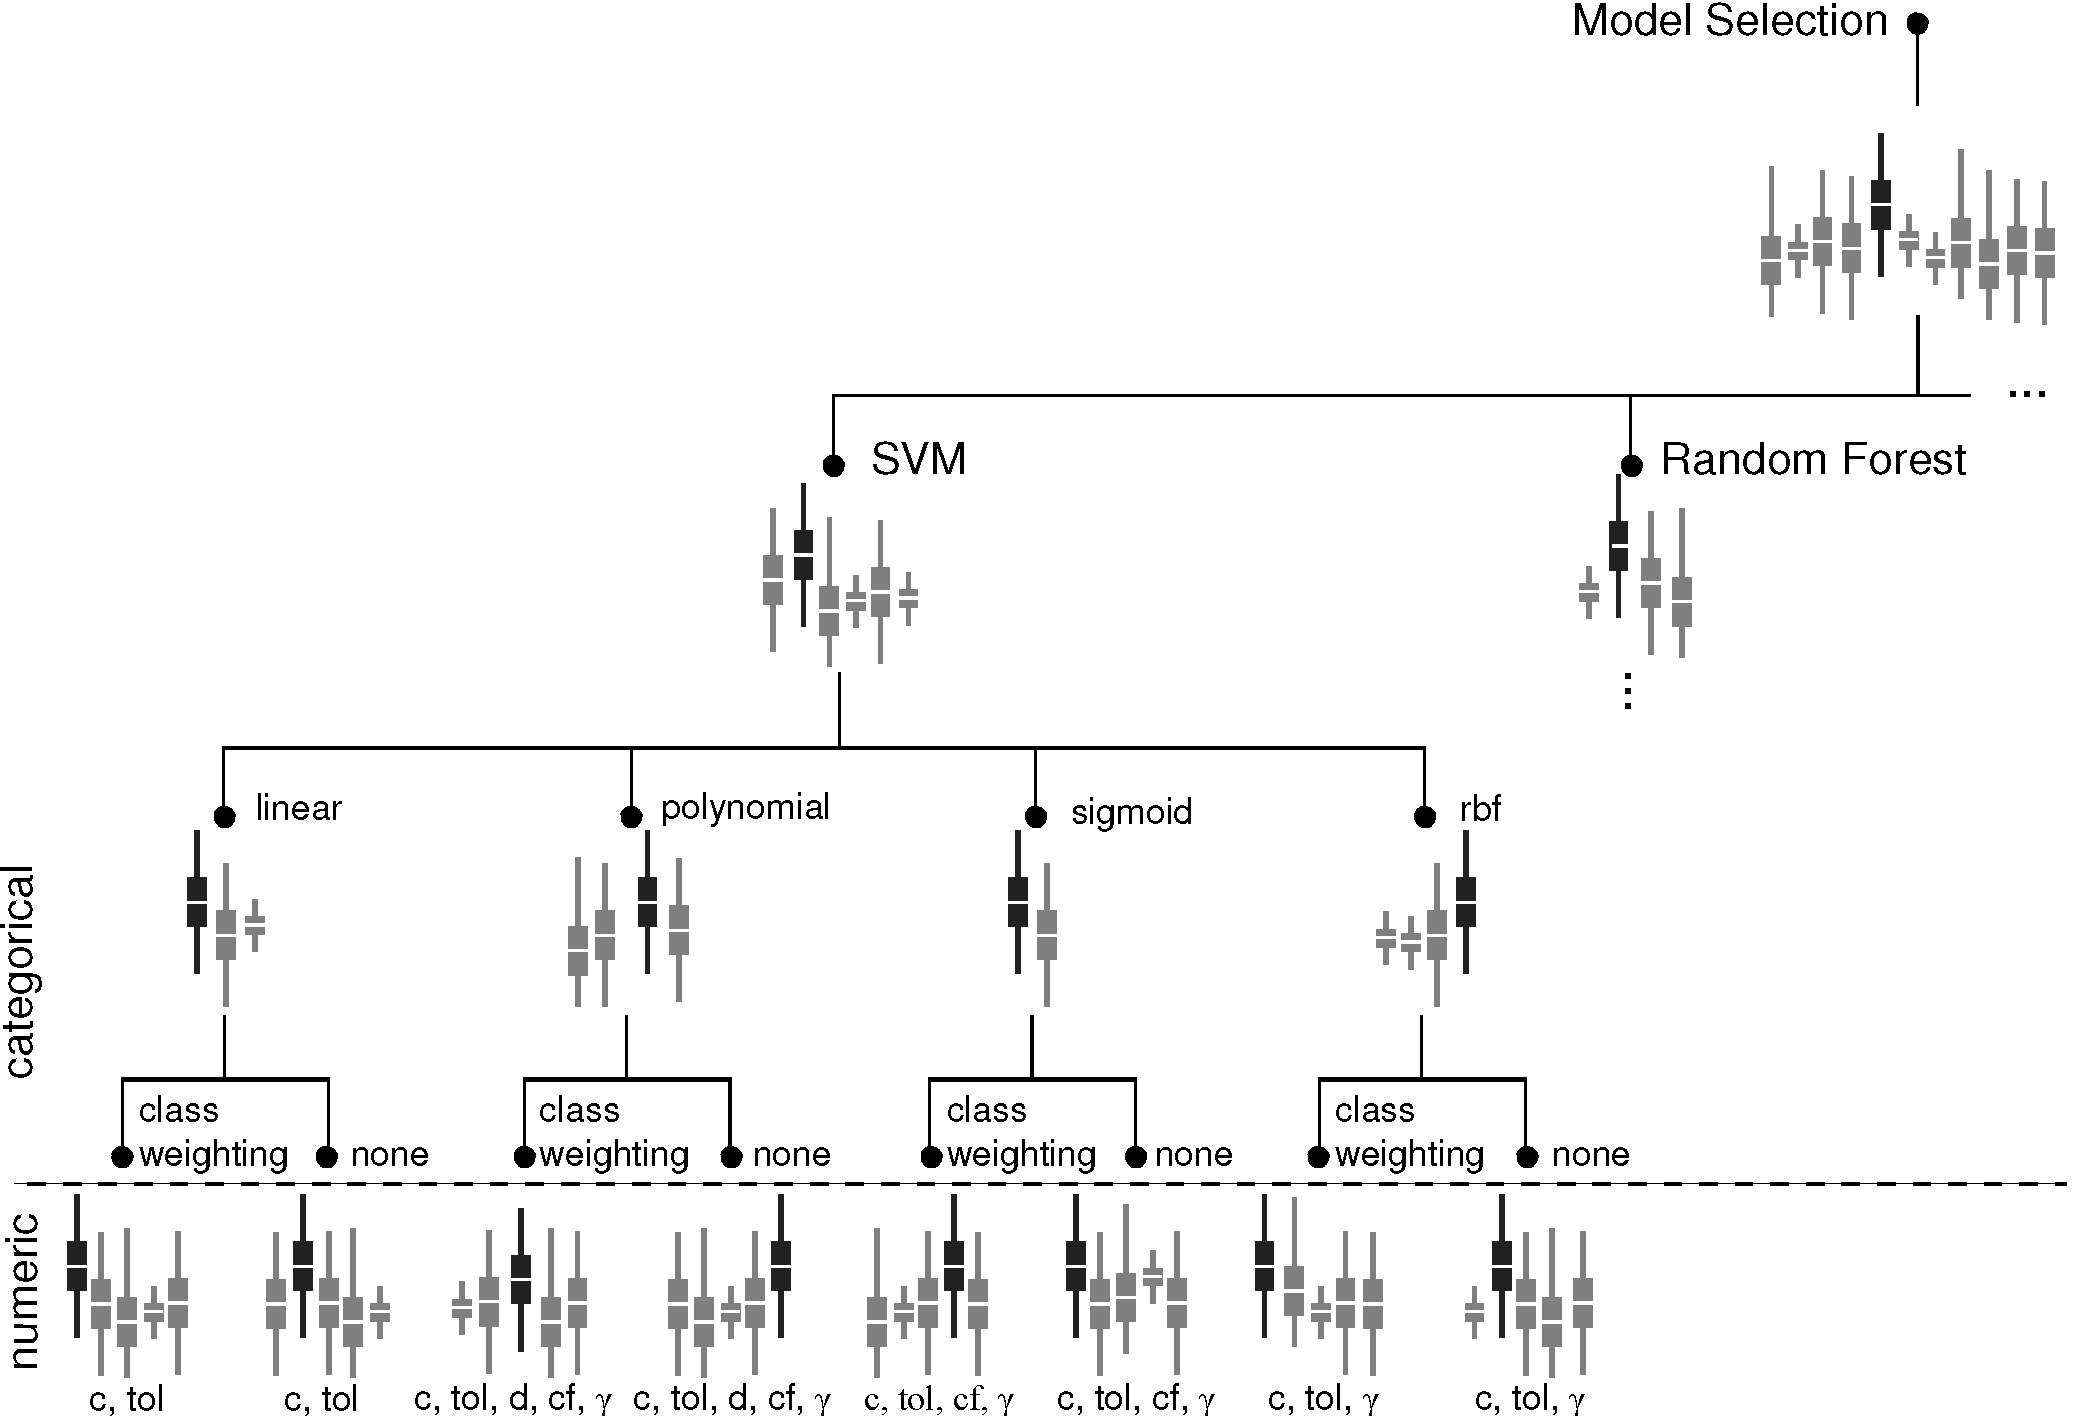
\includegraphics[width=\textwidth]{tree}
	\caption[Hierarchical model selection]{Hierarchical model selection. Each box plot represents
	the distribution of scores for a specific model. Distributions shown in black are promoted
	upwards to subsequently compete against models from the same local hierarchy.}
	\label{img:tree}
\end{figure}

\subsection{Candidate model filtering}
The optimization stage will mostly retrieve models with high performance indices. Most optimization
techniques try to find local optima, and as a consequence, they might end up testing a large number
of configurations close to each optimum. This means that the distribution of hyperparameter values
sampled and evaluated by the optimization stage will tend to have more density around the different
local maxima found. A clustering approach is used here to exploit this fact and retrieve
high-scoring configurations from different local maxima. This avoids overrepresentation of
configurations from a single hill in the score landscape and returns a small number of
configurations that represent more homogeneously the regions that yield good scores.

Clustering the evaluated configurations with the {\bf $k$-means} algorithm is used here to retrieve
$k$ clusters of configurations, and choose the configuration with the highest score from each cluster as
one of the candidate configurations that will represent a specific numerical hyperparameter space.
The number of means has been arbitrarily chosen to $k = 10$ by default but can be modified via a
parameter setting if needed.

\subsection{Statistical analysis}

Given a set of models, the distribution of their scores on different versions of the hold out
dataset is studied to determine which model offers enough evidence to be considered the best one.

Each model is used for prediction on the hold out dataset several times by using $m$ repetitions of
$k$-fold cross-validation ($m=15,~k=2$ by default). A multiple comparison statistical test (MCT) is
applied on the distributions of $m\cdot k$ scores obtained for each model.

Parametric MCTs make use of direct measurements of the data (such as the mean and variance), whereas
non-parametric MCTs rely on comparisons of other properties of the data (e.g. the ranking of the
groups according to some criteria) which makes them more general and applicable to a wider range of
distributions, at the expense of statistical power \cite{sheskin2003statistics}. Parametric
comparison tests are more statistically powerful and are thus preferred over non-parametric
alternatives.  Parametric tests, however, are only valid under certain specific conditions, and when
such conditions are not met, non-parametric comparison tests must be used instead.

The MCTs determine, up to a certain probability $\alpha$, whether there are significant differences between a
group of distributions or not, but do not tell the actual distributions that show differences. A
\emph{post-hoc} test is required in order to find which distributions differ. Both parametric and
non-parametric post-hoc tests exist.

The aim of the statistical analysis in the context of this work is to compare the distributions of
performance indices for all candidate models with respect to the highest-scoring one, and discard
all the candidate models with strong statistical evidence that they perform worse. The models kept
are {\bf score-wise equivalent} to the best one. The overall procedure is based on
\cite{pizarro2002mct} and \cite{demsar2006mct} for significance testing.

The chosen \emph{parametric} MCT is the {\bf one-way ANOVA test} \cite{fisher1925statistical}, which is a
generalization of the $t$-test that corrects for accumulated errors when performing comparisons
between more than two distributions, by comparing a statistic against a $F$-distribution that
considers the specific number of distributions to compare as a parameter.

The one-way ANOVA test can be used when:
\begin{enumerate}
	\item The observations for all the distributions are independent.
	\item The distributions are approximately normal. This is tested by applying the
	{\bf Kolmogorov-Smirnov test} (K-S test, validates that a sample comes from a given distribution) on
	the sample (after standardization) against a standard normal distribution $\mathcal{N}(0,1)$
	\item The distributions have homogeneous variances (homoscedasticity). This is tested by
	applying the {\bf Bartlett's test} \cite{bartlett1937} on the different distributions of scores.
\end{enumerate}

As stated above, a post-hoc test is required when the ANOVA test determines that there are
significant differences between groups of scores. The {\bf Tukey's honest significance test} compares
simultaneously all the groups of scores and informs what groups are significantly different. The
Tukey's test is then used to find the sets of performance indices that are not significantly
different from the the highest-scoring one. Here it is assumed safe to discard models that do not
pass the Tukey's test, and keep the rest for further analysis.

When the conditions to apply the parametric MCT are not met, the {\bf Kruskal-Wallis test} is
applied instead to decide if significant differences exist, and the {\bf Nemenyi test} is used as
the post-hoc test to find the actual significantly different groups in the same way as for the
parametric case.

\subsection{Ranking criteria}
The statistical analysis reduces the number of candidate models to those that statistically perform
as good as the best, according to their performance indices. Other criteria are evaluated on the
selected models in order to compare them and decide which one is the best from a group of score-wise
equivalent models.

The criteria used here are described in table \ref{tab:ranking}. Each criterion is evaluated for each
candidate model, and used for ranking them. Fractional rankings (to account for ties) are weighted by
a user-defined relative importance value and combined into a compound ranking. The top $n$ models
according to this compound ranking are selected.

\begin{table}[here]
	\centering
	\begingroup
	\begin{tabularx}{\textwidth}{| l X |}
	\hline
	Criterion & Description \\
	\hline
	Generalization & Average score of the model on the hold out dataset. Models with greater values
	are preferred.\\
	Speed & Average measured runtime of applying the model on the hold out dataset. Models with
	lower values are preferred.\\ Stability & Measure of variability of the scores for a model
	(standard deviation). Models with lower values are preferred. \\
	Simplicity & Predefined value associated to the SML algorithm. Models with lower values are
	preferred.\\
	Interpretability & Predefined value associated to the SML algorithm. Models with lower values
	are preferred.\\
	\hline
	\end{tabularx}
	\endgroup
	\caption{Alternative ranking criteria for score-wise equivalent models}
	\label{tab:ranking}
\end{table}



for each numerical hyperparameter space:
	find representative local maxima from optimization process
	use m repetitions of k fold cross-validation \todo{find name for this}
	apply statistical test of means
	discard models significantly different to the best
	evaluate other qualities of the selected models \todo{find a name for this}
	rank the models by such criteria and keep the top n
	compare all selected models to the models from the different categories on the same subtree

===============

getselectedmodels (node, n)
if node is numerical hyperparameter space:
	candidate models = select representatives by kmeans
else (is category)
	candidate models = []
	for each category at this level:
		candidatemodels.append(getselectedmodels(category))
selected models = statistically test(candidatemodels)
selected models = top n rank trimmed
return trimmed


The statistical test applied to the model scores compares the mean and spread of the scores
obtained by a single model against all other candidate models. The test is summarized in algorithm
\ref{alg:statistical_test}

param: list of score groups, alpha
if score groups are normal with similar variance:
	use anova to decide if there are significant differences
	if so, apply tuckey test to see 


It is worth noticing that the proportion of data to be used for optimization and for model selection
is defined by the user (a default of 50\% of the data for optimization and 50\% for model selection
is suggested). When dealing with small datasets, the choice of this ratio will affect the
reliability of both optimization and model selection results. Alternative approaches such as
bootstrapping, or overlapping of the optimization and the model selection set may be helpful to some
extent, but should be used cautiously \todo{find a way to say this properly}

Making use of the tree structure for model selection not only provides a very efficient way to
discriminate between model performances, but also has the advantage that it compares models with
similar characteristics, and selects a small but representative subset of the models to compete
against other sets of models.

\subsection{The model selection algorithm}
The process described above can be summarized as shown in algorithm \ref{alg:modelselection}

\begin{algorithm}[here]
	\begin{algorithmic}
		\Function{select\_models}{hyperparameter\_tree, top\_$n$, $\alpha$, $k$}
			\State candidates $\gets \emptyset$
			\If {hyperparameter\_tree is numerical}
				\State candidates $\gets$ \Call{get\_$k$-means}{hyperparameter\_tree, $k$}
			\Else
				\For {category in hyperparameter\_tree}
					\State candidates $\gets$ candidates $\cup$ \Call{select\_models}{category, top\_$n$,
					$\alpha$, $k$}
				\EndFor
			\EndIf
			\State candidates $\gets$ \Call{find\_scorewise\_equivalents}{candidates, $\alpha$}
			\State candidates $\gets$ \Call{get\_top\_$n$}{candidates, ranking\_criteria, top\_$n$}
			\State\Return candidates
		\EndFunction
	\end{algorithmic}
	\caption{Model selection algorithm}
	\label{alg:modelselection}
\end{algorithm}

The function obtains the best models at each level of the hyperparameter hierarchy, by recursively
filtering and selecting the best models from the lower branches of the hierarchy and passing them to
the level immediately above. At the top level, the ranked list of best models will be reported as
the result of the model selection stage.


